\documentclass[DM,lsstdraft,authoryear,toc]{lsstdoc}
\input{meta}

% Package imports go here.
% \usepackage{blindtext}

\usepackage{booktabs}


\usepackage[colorinlistoftodos]{todonotes}
\let\Oldtodo\todo
\renewcommand{\todo}[1]{\Oldtodo[inline]{#1}}
\newcommand{\eric}[2][]{\Oldtodo[inline,color=cyan, #1]{Eric: #2}}
\newcommand{\ian}[2][]{\Oldtodo[inline,color=green, #1]{Ian: #2}}
\newcommand{\sean}[2][]{\Oldtodo[inline,color=yellow, #1]{Sean: #2}}


% Local commands go here.

%If you want glossaries
%\input{aglossary.tex}
%\makeglossaries

\title{DECam Templates for LSST Alert Production}

% This can write metadata into the PDF.
% Update keywords and author information as necessary.
\hypersetup{
    pdftitle={DECam Templates for LSST Alert Production},
    pdfauthor={Sean PatrickMacBride},
    pdfkeywords={}
}


% Optional subtitle
% \setDocSubtitle{A subtitle}

\input{authors}

\setDocRef{DMTN-362}
\setDocUpstreamLocation{\url{https://github.com/lsst-dm/dmtn-362}}

\date{\vcsDate}

% Optional: name of the document's curator
% \setDocCurator{The Curator of this Document}

\setDocAbstract{%
In this technote, we describe the implementation of a plan for using archival images from the Dark Energy Camera to make template images for image differencing against LSST-Camera images. We discuss the inception of this processing campaign, image selection and curation criteria, the plan for staged deployment, and expectations for the characteristics of Rubin-DECam alerts.
}

% Change history defined here.
% Order: oldest first.
% Fields: VERSION, DATE, DESCRIPTION, OWNER NAME.
% See LPM-51 for version number policy.
\setDocChangeRecord{%
  % \addtohist{1}{YYYY-MM-DD}{Unreleased.}{MacBride}
  \addtohist{1}{2026-11-17}{Revision to \textit{DECam Templates}, \textit{Image Selection}, and \textit{Alert Expectations} chapters.}{MacBride}
}


\begin{document}

% Create the title page.

\maketitle
% Frequently for a technote we do not want a title page  uncomment this to remove the title page and changelog.
% use \mkshorttitle to remove the extra pages

% ADD CONTENT HERE
% You can also use the \input command to include several content files.

\section{DECam Templates}\label{sec:inception}
 
\subsection{Motivation}
 
Rubin alert production requires a template image at every sky position in every band in which alerts are to be distributed. 
The baseline plan for the Early Science Program was to build these templates incrementally from LSSTCam data, first from commissioning observations, and then from images accumulated during the first year of the survey \citep{DMTN-107,RTN-011}. 
As of Nov. 2026, commissioning observations processed as part of Data Preview 2 have comprised the bulk of the templates deployed to alert production.
Survey-strategy simulations indicate that a first year affected by strong El Ni\~no weather, hardware downtime, and ongoing engineering activities, would not quickly deliver templates across the WFD area.

Two mitigations for this shortfall have been considered within the survey strategy team: a dedicated high-priority \textit{template tier} in the scheduler that targets template-quality visits, and the use of shorter (20\,s) exposures to accumulate visits faster. Both carry costs to the nominal survey footprint, band balance, data-processing, and cadence. A third, complementary option, is to build templates from archival data that already exists.


Scientifically, the scheduling of the planned IR1 LIGO-Virgo-Kagra during the first year of the survey motivated us to consider all available options to enable templates were available over a wide survey area.
The LIGO--Virgo--KAGRA (LVK) Intermediate Run~1 (IR1), a planned six-month observing run with both LIGO detectors online and Virgo and KAGRA joining as available, is currently expected to begin in mid-January 2027. With sensitivity comparable to the fourth observing run, IR1 should deliver compact-binary detections every few days, a subset of which may involve neutron stars and produce kilonovae \citep{igwn_observing_plans_2026}. This makes IR1 a rare opportunity for Rubin Observatory: its wide field of view and depth are well matched to the large localization regions of gravitational-wave events, and the faint, fast-fading optical counterparts are precisely the sources that a deep, multi-band survey telescope is best placed to find and characterize. With detection and characterization, high-impact scientific opportunities in cosmology, transient astrophysics, and nuclear physics are enabled during coincident operations.

Realizing that potential, however, depends on difference imaging, and difference imaging requires templates. LSSTCam templates will cover only a small fraction of the sky when IR1 begins, so over most candidate localization regions a counterpart search would lack the reference images needed to detect new sources in real time. Templates built from archival DECam data fill this gap across much of the southern sky in $griz$, and they matter for the science as well as the coverage: the $g$-band templates in particular enable the color information needed to discriminate kilonovae from other fast transients. Having vetted DECam templates deployed in Rubin Alert Production before IR1 begins is therefore essential to turning Rubin's ToO capability into alerts that the gravitational-wave community can act on.
 
The Dark Energy Camera (DECam) on the Blanco telescope has imaged a large fraction of the southern sky in multiple bands through public surveys including DES, DELVE and other surveys \citep{DES,DELVE}. Its filters are similar (but not identical) to the Rubin $g$, $r$, $i$ and $z$ bands, and its pixel scale (0.263\,arcsec) is within a factor of 1.5 of LSSTCam's (0.2\,arcsec). Archival DECam exposures offer a route to templates that does not depend on the LSSTCam image accumulation described above.
 
Several limitations shape how these templates can be used.
\begin{itemize}
  \item \textbf{Alert production only.} DECam-based templates are a stopgap for AP. They will not be used for Data Release Production (DRP), which requires complete LSSTCam coverage to enable difference imaging in future data releases.
  \item \textbf{Band coverage.} The $u$-band system response of DECam differs from Rubin's significantly. This campaign targets $griz$ only.
  \item \textbf{Epoch and instrument differences.} The archival images are many years older than the Rubin science images, so stars with appreciable proper motion subtract as dipoles. In many ways, this is a good diagnostic for astrometric precision.
\end{itemize}

Whether to retain or drop the template tier and shorter exposures is a decision for the Survey Cadence Optimization Committee (SCOC) and is outside the scope of this note.

\subsection{Previous Work: Rubin--DECam differencing in COSMOS (spring 2026)}
 
A first end-to-end test was carried out in spring 2026 by members of the AP team. Archival DECam exposures of the COSMOS field already available at the USDF were run through the Science Pipelines using the \texttt{QuickTemplate} pipeline in \texttt{ap\_pipe}, which performs single-frame processing, builds warps, and assembles coadds. The templates used the same \texttt{lsst\_cells\_v2} skymap as the Rubin templates, and the resulting coadds were then differenced against LSSTCam visits taken in early 2026.
 
The outcome was encouraging, but clearly showed work remaining. For a representative visit and detector in $g$ band, all clearly real transients and moving objects that were detected with Rubin--Rubin differencing were also detected at high reliability with the DECam template. However, roughly 20 times as many unfiltered diaSources were produced, and about 4 times as many passed the standard quality and reliability cuts. 
While there are a variety of reasons to expect a larger number of ``real'' detections in differences with DECam templates (\S \ref{sec:alerts}), the excess diaSources showed strong spatial clustering indicative of problems in the image subtraction.
This performance was judged unsuitable for production deployment due to the high rate of false positives.
%The excess was attributed to proper motion between the DECam and Rubin epochs, poorer template seeing, bandpass differences, and an apparent underestimate of the difference-image variance leading to spurious detections on correlated noise. Restricting to a reliability of 0.9 or higher retained most real moving objects and transients, but at the cost of variable star source detection.

This issue was identified as arising from noise correlations introduced during the warping of the DECam template to the Rubin science image, which was exacerbated by the difference in pixel scale between the two cameras.
By accounting for this difference, the spatial structure in the detected diaSources was greatly reduced. 
\ian{Review this summary and expand if desired}
 
\subsection{Previous Work: Target-of-Opportunity follow-up}
 
At the same time, the Rubin ToO program faced a closely related problem, as no LSSTCam templates exist over most of the sky. The ToO follow-up of the S251112cm event included a pilot comparison of Rubin--DECam and Rubin--Rubin differencing over a $\sim$30\,deg$^2$ region. Note that for this analysis, the DECam templates that were used for this analysis were coadd level images processed by the DESDM pipeline \citep{Morganson_2018}, which differs from the LSST science pipelines. 

The Rubin-DECam differences produced 5-8 times more \texttt{diaSources} per epoch than the Rubin-Rubin differences, and for that analysis, the Rubin-Rubin differences were judged the cleaner option where a suitable earlier Rubin epoch existed. However, this limited the scope of analyses in this context, as one Rubin visit had to be designated the \textit{template} for the purpose of DIA.

\eric{Comment on challenges of ad-hoc processing motivating AP templates}

% ECB: I think this bears a little more thinking
%While this ToO image processing campaign was challenging, it elucidated a principle we adopt for this campaign: DECam templates are for locations where LSSTCam templates are not available. Where LSSTCam templates exist, we deploy them to Rubin AP.
\todo{we should describe why we though reprocessing was important given the prior use of DESDM images}
 
\subsection{Launch of the Wide-Area Campaign}

 
The campaign to produce DECam templates for Rubin AP in a wide-area was launched in early August 2026. At kickoff, we devised a prototype pipeline above together with the issues that needed to be settled before wide-area template production could begin:
\begin{enumerate}
  \item The \texttt{SPIKE} mask, tuned for Rubin images and somewhat over-aggressive for DECam;
  \item The reference catalogs used for astrometric and photometric calibration;
  \item The choice of skymap, in particular whether one matched to the DECam pixel scale would reduce correlated noise, versus the convenience for Prompt Processing of a skymap shared with the Rubin templates;
  \item Whether the visit-selection algorithm used for deep coadds is the best fit for DECam data;
  \item The underestimated variance in the DECam-template difference images, which caused spurious detections on correlated noise, and whether to correct the variance calculation or raise the detection threshold.
\end{enumerate}
 
Following kickoff, we established the pipeline configuration to build on \texttt{QuickTemplate}, and ELAIS-S1 was chosen as the pilot region. 
 
\subsection{From pilot to survey-scale processing}
 
The pilot region was processed at NERSC through autumn 2026 with three template-selection configurations compared using PSF-variation metrics, and on the quality of the resulting difference images. Rubin-DECam difference images made from the pilot templates were judged to be satisfactory, and an independent check against \textit{Gaia} showed that stars with proper motions down to roughly 10\,mas\,yr$^{-1}$ appear as dipoles in the diaSources, with the measured dipole lengths in excellent agreement with the \textit{Gaia} values (see Figure~\ref{fig:gaia_pms}).

With the pilot validated, the campaign moved to sky-area \textit{chunks} processed at NERSC (see Figure~\ref{fig:chunk_schem}), transferred to the USDF, and vetted before any deployment to the embargo repository. The first of these, chunk~0, was produced in early November 2026 and ingested at the USDF on 5~November 2026, and were deemed satisfactory to deploy to Rubin AP on Nov. 10. % The criteria applied to select and curate input images are described in Section~2, the plan for staged deployment in Section~3, and expectations for alert volume and reliability scoring in Section~4.

 
\subsection{Guiding Principles}
 
The following principles have guided the campaign from its inception, and several are enforced in the template curation and deployment process.
\begin{itemize}
  \item DECam templates serve AP only and are used only where LSST templates do not exist.
  \item For each tract and band, the official template collection used in real-time processing contains one style of template, Rubin or DECam, never both.
  \item DECam templates are ingested under a distinct dataset type, \texttt{template\_coadd\_decam}, and processed with a dedicated top-level AP pipeline, so that provenance is unambiguous in the resulting alert products.
  \item Template production targets the $griz$ bands.
\end{itemize}
\newpage
\section{Image Selection}

\label{sec:selection}

\subsection{Overview}

Roughly half a million DECam exposures cover the southern sky. Most are not suitable inputs for alert-production templates: many were taken in poor atmospheric or instrumental conditions, some suffer from tracking failures or severe optical ghosts, and the depth and image quality of the archive are highly inhomogeneous. Selecting which exposures to reprocess is therefore the first step in the campaign, and it determines both the area that can be covered and the quality of the resulting templates.

This section describes how the input exposures were chosen. In brief, the parent list of exposures comes from the curated exposure list that the DELVE team uses for DELVE DR3 (\cite{DELVE})\footnote{Note: DELVE DR3 publication is in-prep, DR2 publication is provided for reference. More information about DR3 is available from \href{https://datalab.noirlab.edu/data/delve#delve-dr3}{datalab.noirlab.edu/data/delve#delve-dr3}}; a DELVE-maintained exclusion list removes known problem exposures and CCDs, and a per-template selection step picks the best-seeing exposures for each position. Table~\ref{tab:criteria} summarizes the criteria, which are described in detail below.

\subsection{Parent exposure list from DELVE DR3}

The campaign adopted the exposure list used by DELVE to generate its DR3 catalog-level coadds. This is a different product from the DELVE image coadds released previously using the DESDM pipeline.
The input list is combined with DELVE's DECam exclude list, which compiles several classes of artifact and problem exposure into a single file. Some entries are visits or CCDs that should always be excluded, such as those affected by tracking problems. Others, notably CCDs with prominent optical ghosts, may reasonably be included or excluded depending on the use. In the ELAIS-S1 pilot, for example, two visits in which more than 30 CCDs were ghosted were dropped by hand, and the chunk production used the explicit visit-detector combinations provided by the exclusion list. The input visits per band are shown in Figure~\ref{fig:delve_vis_nomask}.

\begin{figure}
    \centering
    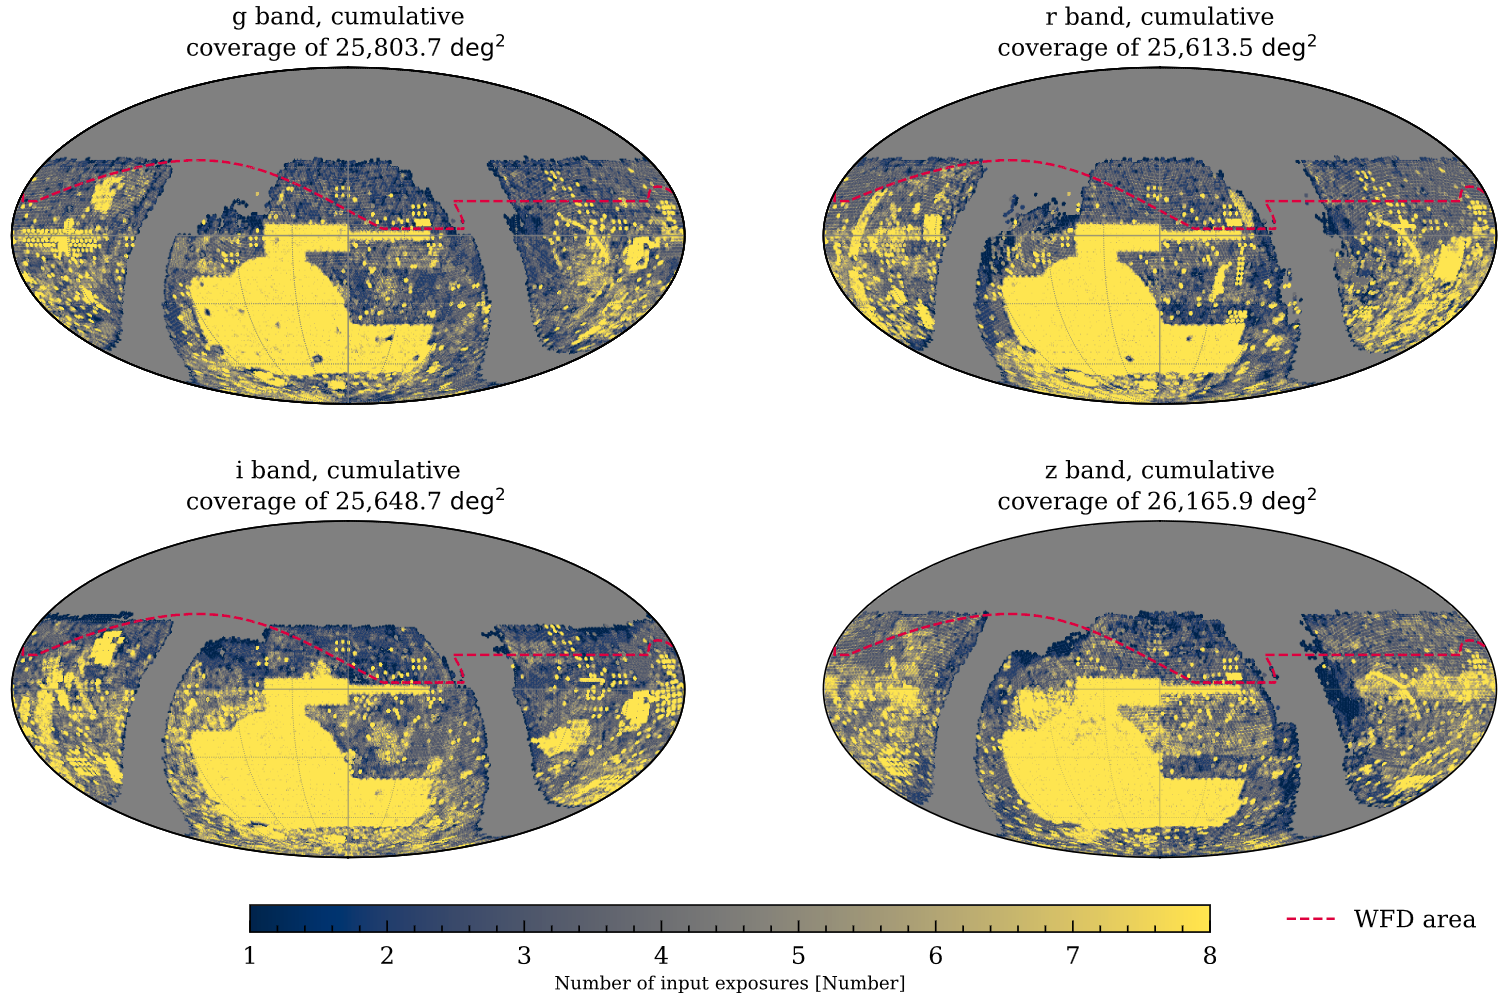
\includegraphics[width=0.99\linewidth]{figures/DELVE_vis_nomask.png}
    \caption{Input visits from DELVE DR3 shown per band, with the WFD northern declination limit shown in dashed red line.}
    \label{fig:delve_vis_nomask}
\end{figure}

\subsection{Band and footprint selection}

\textbf{Bands.} The campaign targets $griz$ only. The DELVE input lists are provided for these four bands. % DECam $u$-band data are sparse over most of the sky, and $Y$-band data exist almost exclusively in DES. Moreover, the DECam $u$-band system response differs appreciably from Rubin's, which would complicate its use even where data exist.

\textbf{Footprint.} Processing is limited to declinations south of approximately $+30^\circ$, which extends beyond the nominal Rubin wide-fast-deep and ecliptic regions so that templates would be available should LSST observations be taken outside the main footprint. A Galactic-latitude mask of $|b|>10^\circ$ is also applied to the DELVE inputs. Coverage was assessed against maps of where LSSTCam has accumulated enough images that templates could be built independent of this campaign already (\textit{incremental template maps}), so that DECam processing prioritizes regions in which LSSTCam templates are unlikely to be available. 

With these cuts, the potential template area is of order $6\times 10^4$\,deg$^2$ summed over $griz$, of which around $4\times 10^4$\,deg$^2$ is in seasonally prioritized regions, with a smaller requirement in $z$ band where Rubin already has substantial incremental template coverage. These estimates apply the general footprint cuts and do not yet fold in the true DELVE coverage, so the achievable area will be somewhat smaller.

% \sean{add a figure here showing the DECam coverage with the incremental mask applied}

Some regions are covered only partially or not at all by this input list. The Large and Small Magellanic Clouds are included in the input dataset. The part of the North Ecliptic Spur that passes through Orion and the Flame nebula is uncovered, but it suffers high extinction and has been de-prioritized by extragalactic surveys. Other DECam programs, such as DECaPS in the Galactic plane, provide additional images, but they would require different processing and are deferred until the present campaign is complete.

\subsection{Selection of exposures for each template}

Beyond the parent list, a visit-selection step in the template pipeline chooses the exposures that enter each template. The pipeline is derived from the base DECam \texttt{QuickTemplate} pipeline in \texttt{ap\_pipe}. Early tests used its default best-seeing selection. A quantile-based selector was initially adopted, with a maximum PSF FWHM of 1.8 arcsec, a minimum of eight visits, and a seeing quantile cut at 0.5. Experience showed that quantile-based selection has little effect until roughly ten or more images per band are available, and that DECam inputs per position are often too few for it to take effect, so the emphasis shifted from selecting the best fraction of inputs to simply rejecting poor ones.

The pilot compared three configurations: the earlier default selection, and a best-seeing selection of six exposures with a PSF cut at 1.8 arcsec and at 1.5 arcsec. Based on the PSF-variation metrics and difference-imaging tests, the campaign settled on the following rule: \textbf{each template is built from at most six DECam exposures, taken from the best-seeing exposures that satisfy a PSF cut of 1.5\,arcsec on the individual exposures}. A template is still built when fewer than six qualifying exposures exist, in which case all of them are used.

% \sean{Show plot comparing 1.8 and 1.5 arcsec template quality here}

These quality criteria are applied independently of those that will be used to select LSSTCam images for Rubin templates. The two sets of cuts are not coupled, and the DECam cuts should not be taken as a prediction of the LSSTCam template requirements.

\subsection{Calibration inputs for the selected exposures}

The selected exposures are reprocessed from raw images in the Rubin Science Pipelines. This replaces, rather than reuses, earlier DECam reductions such as the instrumental-signature-removed (instcal) images from the DECam Community Pipeline or the final-cut images from DES data management. Bad-pixel masks, the linearizer and other curated calibrations come from \texttt{obs\_decam}; the defects originate from DES.

Biases and flats were rebuilt from raw calibration exposures on a yearly epoch, and assembled with the pipeline's calibration-production tasks. Fringe frames are built after the $z$-band flats are validated. Because calibrations transferred between pipelines (or versions of the same pipeline) are unreliable, photometric zero points are not imported from DES or DELVE; instead, astrometry and photometry are calibrated against The Monster reference catalog within the Rubin pipeline \citep{DMTN-277}.

Calibration epochs were initially defined to follow a yearly cadence. However, work is ongoing to follow the DES and DECADE epochs, which are determined by instrumental features including power cycles and movements of the filters.

% Two known data issues are accommodated rather than corrected: the headers' read noise values were wrong by factors of roughly 1.5--2 on one backplane for an extended period (approximately 2014 to 2026), which has little effect on broad-band images of reasonable exposure time \todo{confirm the date range and which backplane}, and 
Edge bleeds were identified as a source of artifacts, for which a masking task was developed and validated against the DES edge-bleed mask, raising amplifier-level completeness from 63\% to 90\%. The brighter-fatter correction was judged unnecessary for template production, since the effect is small for this application.

\subsection{Curation and consistency with Rubin templates}

Each template is checked against PSF-variation metrics across tracts and bands before deployment, and the selection and vetting workflow is described in Section~\ref{sec:deployment}. Two curation rules are fixed in advance. First, within any tract and band, the official template collection used for real-time processing contains only one style of template, Rubin or DECam, never a mixture; this is enforced during curation using the expected Rubin coverage described above. Second, DECam templates are ingested under their own dataset type, \texttt{template\_coadd\_decam}, so that the provenance of every template is explicit. The instrument used in the coaddition is also recorded in the template metadata so that difference imaging and downstream products can identify which kind of template was used.


% ---------------------------------------------------------------------------
\begin{table}[t]
\centering
\small
\begin{tabular}{@{}p{0.15\textwidth}p{0.5\textwidth}p{0.25\textwidth}@{}}
\toprule
Stage & Criterion & Source \\  \hline  \hline
\midrule
Parent list & DELVE DR3 exposure list, $griz$ only & DELVE \\ \hline
% Homogenization & Low-quality exposures removed where exposures per band greatly exceed the typical depth (threshold of order 20) & DELVE \\
Exclusion & Known tracking, artifact and ghost-affected visits and CCDs & DELVE exclude list \\ \hline
Footprint & $\delta < +30^\circ$, Galactic-latitude mask, prioritized by expected LSSTCam template coverage & DELVE exposure list \\ \hline
Per-exposure quality & PSF cut of 1.5\,arcsec on individual exposures & Pilot comparison \\ \hline
Per-template selection & Up to six best-seeing exposures; fewer allowed & Pilot comparison \\ \hline
Calibration & Raw reprocessing, rebuilt calibrations by epoch, \textit{The Monster} for astrometry and photometry & Rubin Science Pipelines \\ \hline
Consistency & One template style per tract and band; \texttt{template\_coadd\_decam} dataset type & Deployment plan \\
\bottomrule
\end{tabular}
\caption{Summary of image selection and curation criteria.}
\label{tab:criteria}
\end{table}
\newpage
\section{Deployment Plan}\label{sec:deployment}

Producing templates at survey scale requires many processing steps and substantial data movement, the quality of the output varies across the sky, and the templates must integrate cleanly with the existing LSSTCam template workflow in PP. The campaign therefore proceeds in discrete stages, so that templates are deployed for regions where they are ready, while later regions are still being processed or validated. The regular-processing deployment described here is distinct from the use of DECam templates for ToO analyses. It covers the templates used by PP for real-time alert production, with the expectation that deployment proceeds chunk by chunk as each chunk is processed and vetted.

Chunks are processed with a priority assigned based on field availability. For this reason, we initiated the processing campaign with templates within the DELVE footprint along an RA$=315^\circ$. This region was given priority given the original start date of LVK IR1, which was mid-November 2026\footnote{Note: The announced start date of LVK IR1 as of \today\ is \href{https://observing.docs.ligo.org/plan/\#ligo-virgo-and-kagra-observing-run-plans}{mid-January 2027}}, and the fields available to Rubin at that time. For this reason, we define chunk 0 as the chunk centered at RA$=315^\circ$, DEC$=+15^\circ$, shown in Figure~\ref{fig:chunk_schem}.

\begin{figure}[b!]
     \centering
     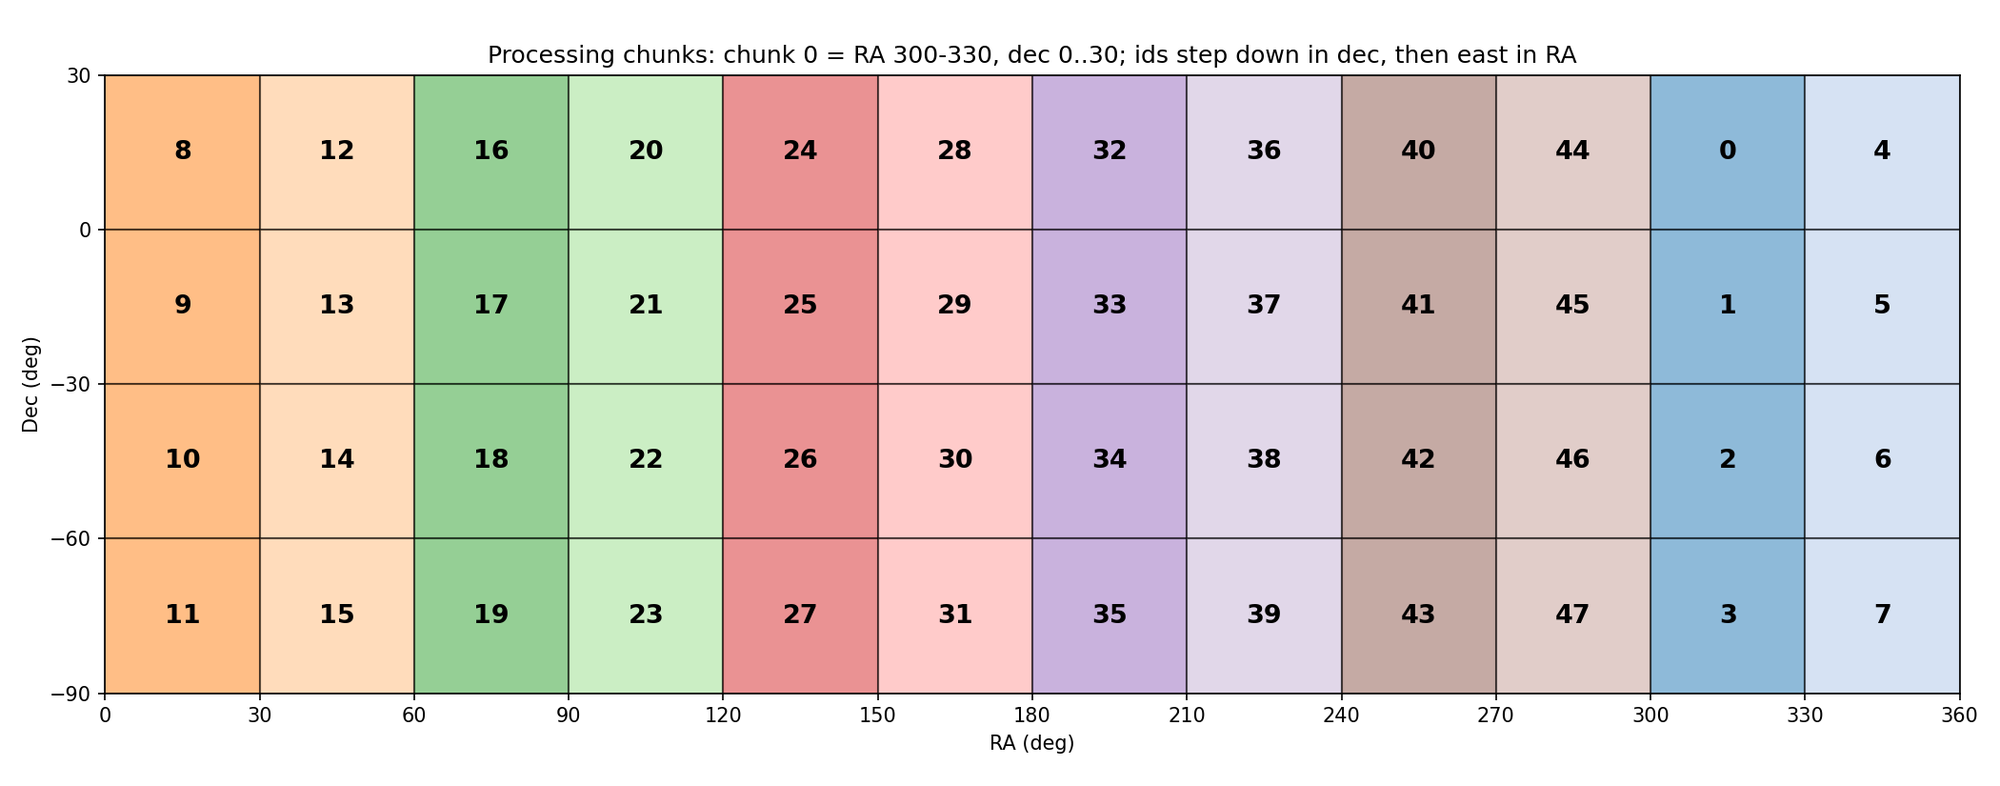
\includegraphics[width=\linewidth]{figures/chunk_schematic.png}
     \caption{A schematic of the chunks across the sky, illustrating the staging of template production and deployment.}
     \label{fig:chunk_schem}
 \end{figure}

\subsection{Transition to LSSTCam templates}

DECam templates are a stopgap, so the deployment plan includes their eventual replacement. As LSSTCam accumulates enough images in a tract and band, a decision is needed on when that tract and band switches from a DECam template to an LSSTCam template. Because only one style of template exists in the official chain for a given tract and band, the switch is a curation step rather than a runtime choice. \cite{RTN-133} quantifies how the benefit of DECam templates depends on the open choices: the number of visits per LSSTCam template, the latency of template builds, the image-quality cuts on the LSSTCam visits, and the time at which a tract switches from DECam to LSSTCam. The metadata recorded during coaddition is intended to allow a balanced mixture of DECam and LSSTCam templates as this transition progresses.

\subsection{Data retention and archiving}
\label{sec:archiving}

We archive \texttt{template\_coadd}, \texttt{preliminary\_visit\_image}, and \texttt{preliminary\_visit\_summary} datasets to tape at NERSC for each chunk, in the event of re-processing or data reuse for other scientific applications.

\subsection{Current status}

As of \today, chunk~0 (about 500\,deg$^2$) has been produced at NERSC, transferred to the USDF, vetted, re-ingested under the PP-required dataset type, and chained into the curated collection, with tracts and bands overlapping existing LSSTCam coverage removed. The remaining steps for chunk~0 are the transfer to \texttt{embargo}, which requires adjusting file ownership so that the PP service account can create the links, and configuring PP to use the new collection. Processing of other chunks is underway. The status of chunk processing is shown in Table ~\ref{tab:chunks}.

\begin{longtable}{c c c p{2cm} p{2cm} p{3cm}}
\caption{The status of chunk processing, as of \procDate}\label{tab:chunks}\\
\toprule
Chunk & RA range (deg) & Dec range (deg) & Area (deg$^2$) & MJD range (per band) & Expected date of transfer to USDF \\
\midrule
\endfirsthead
\toprule
Chunk & RA range (deg) & Dec range (deg) & Area (deg$^2$) & MJD range (per band) & Expected date of transfer to USDF \\
\midrule
\endhead
\midrule
\multicolumn{6}{r}{\emph{Continued on next page}} \\
\endfoot
\bottomrule
\endlastfoot
0  & 300--330 & $0$ to $30$    & & & \\
1  & 300--330 & $-30$ to $0$   & & & \\
2  & 300--330 & $-60$ to $-30$ & & & \\
3  & 300--330 & $-90$ to $-60$ & & & \\
4  & 330--360 & $0$ to $30$    & & & \\
5  & 330--360 & $-30$ to $0$   & & & \\
6  & 330--360 & $-60$ to $-30$ & & & \\
7  & 330--360 & $-90$ to $-60$ & & & \\
8  & 0--30    & $0$ to $30$    & & & \\
9  & 0--30    & $-30$ to $0$   & & & \\
10 & 0--30    & $-60$ to $-30$ & & & \\
11 & 0--30    & $-90$ to $-60$ & & & \\
12 & 30--60   & $0$ to $30$    & & & \\
13 & 30--60   & $-30$ to $0$   & & & \\
14 & 30--60   & $-60$ to $-30$ & & & \\
15 & 30--60   & $-90$ to $-60$ & & & \\
16 & 60--90   & $0$ to $30$    & & & \\
17 & 60--90   & $-30$ to $0$   & & & \\
18 & 60--90   & $-60$ to $-30$ & & & \\
19 & 60--90   & $-90$ to $-60$ & & & \\
20 & 90--120  & $0$ to $30$    & & & \\
21 & 90--120  & $-30$ to $0$   & & & \\
22 & 90--120  & $-60$ to $-30$ & & & \\
23 & 90--120  & $-90$ to $-60$ & & & \\
24 & 120--150 & $0$ to $30$    & & & \\
25 & 120--150 & $-30$ to $0$   & & & \\
26 & 120--150 & $-60$ to $-30$ & & & \\
27 & 120--150 & $-90$ to $-60$ & & & \\
28 & 150--180 & $0$ to $30$    & & & \\
29 & 150--180 & $-30$ to $0$   & & & \\
30 & 150--180 & $-60$ to $-30$ & & & \\
31 & 150--180 & $-90$ to $-60$ & & & \\
32 & 180--210 & $0$ to $30$    & & & \\
33 & 180--210 & $-30$ to $0$   & & & \\
34 & 180--210 & $-60$ to $-30$ & & & \\
35 & 180--210 & $-90$ to $-60$ & & & \\
36 & 210--240 & $0$ to $30$    & & & \\
37 & 210--240 & $-30$ to $0$   & & & \\
38 & 210--240 & $-60$ to $-30$ & & & \\
39 & 210--240 & $-90$ to $-60$ & & & \\
40 & 240--270 & $0$ to $30$    & & & \\
41 & 240--270 & $-30$ to $0$   & & & \\
42 & 240--270 & $-60$ to $-30$ & & & \\
43 & 240--270 & $-90$ to $-60$ & & & \\
44 & 270--300 & $0$ to $30$    & & & \\
45 & 270--300 & $-30$ to $0$   & & & \\
46 & 270--300 & $-60$ to $-30$ & & & \\
47 & 270--300 & $-90$ to $-60$ & & & \\
\end{longtable}
\newpage
\section{Alert Expectations} \label{sec:alerts}


In this section we highlight issues alert users may wish to be aware of.


\subsection{Identifying Alerts with DECam Templates}

Starting in alert schema v11.2, we added several columns to the diaSource table to enable users to recognize when alerts come from difference images generated from DECam templates. 
They are:

\eric{summarize}

\subsection{Alert Rates}

\todo{summarize pilot}

\subsection{Expected Origins of Additional DiaSources}

DiaSources originate in positive and negative $5\sigma$ excesses in the difference images.
While Real/Bogus scoring \citep{DMTN-337} attempts to ensure that the resulting alerts that result are astrophysical, the classifier is ultimately morphological in nature.  
We note several cases where Rubin$-$DECam will generate more diaSources than Rubin$-$Rubin for the same science image:

\subsection{Bandpass Differences}

Sources with extreme colors may appear as diaSources due to differences in the net filter throughput.
Absent other variability, these sources will have constant difference image flux and and be filtered using timeseries features.

\todo{would be nice to make a plot or so here showing what counts as extreme}

\subsection{Stellar Proper Motion}

% Many stars will exhibit proper motions between the epoch of the DECam template and the current Rubin image.
% In difference images, these will appear as dipoles with positive and negative lobes.
% The `isDiplole` flag may be used to efficiently remove such sources, which are also typically given lower scores by Real/Bogus.
% Users interested in proper motions may make use of the dipole fit parameters and the template epoch information provided.
We find that many new dipoles detected in Rubin-DECam difference images, including those with high reliability scores, are not transients or artefacts of subtraction, but rather represent true astrophysical motion of stars. The DECam templates are built from exposures taken about a decade before the Rubin visits, so any star whose proper motion over that interval is comparable to the PSF width leaves a dipole in the difference images. We crossmatched all \texttt{diaSources} from the Rubin-DECam difference images to Gaia DR3 and selected those with a successful dipole fit and a Gaia proper motion, giving 46 dipoles. The measured dipole length, \newline $\texttt{ip\_diffim\_DipoleFit\_separation}$ (or $\texttt{dipoleLength}$ in the APDB), agrees with the expected displacement of the star, Gaia proper motion multiplied by the interval between the epoch of the DECam template and the current Rubin image ($\approx$10.62 years), in magnitude (figure \ref{fig:gaia_pms}) as well as in direction. Thus, we recommend that the users interested in extragalactic transients or variable stars to make use of the Gaia proper motion catalog to identify and remove stars that will lead to dipoles.
\begin{figure}[h]
    \centering
    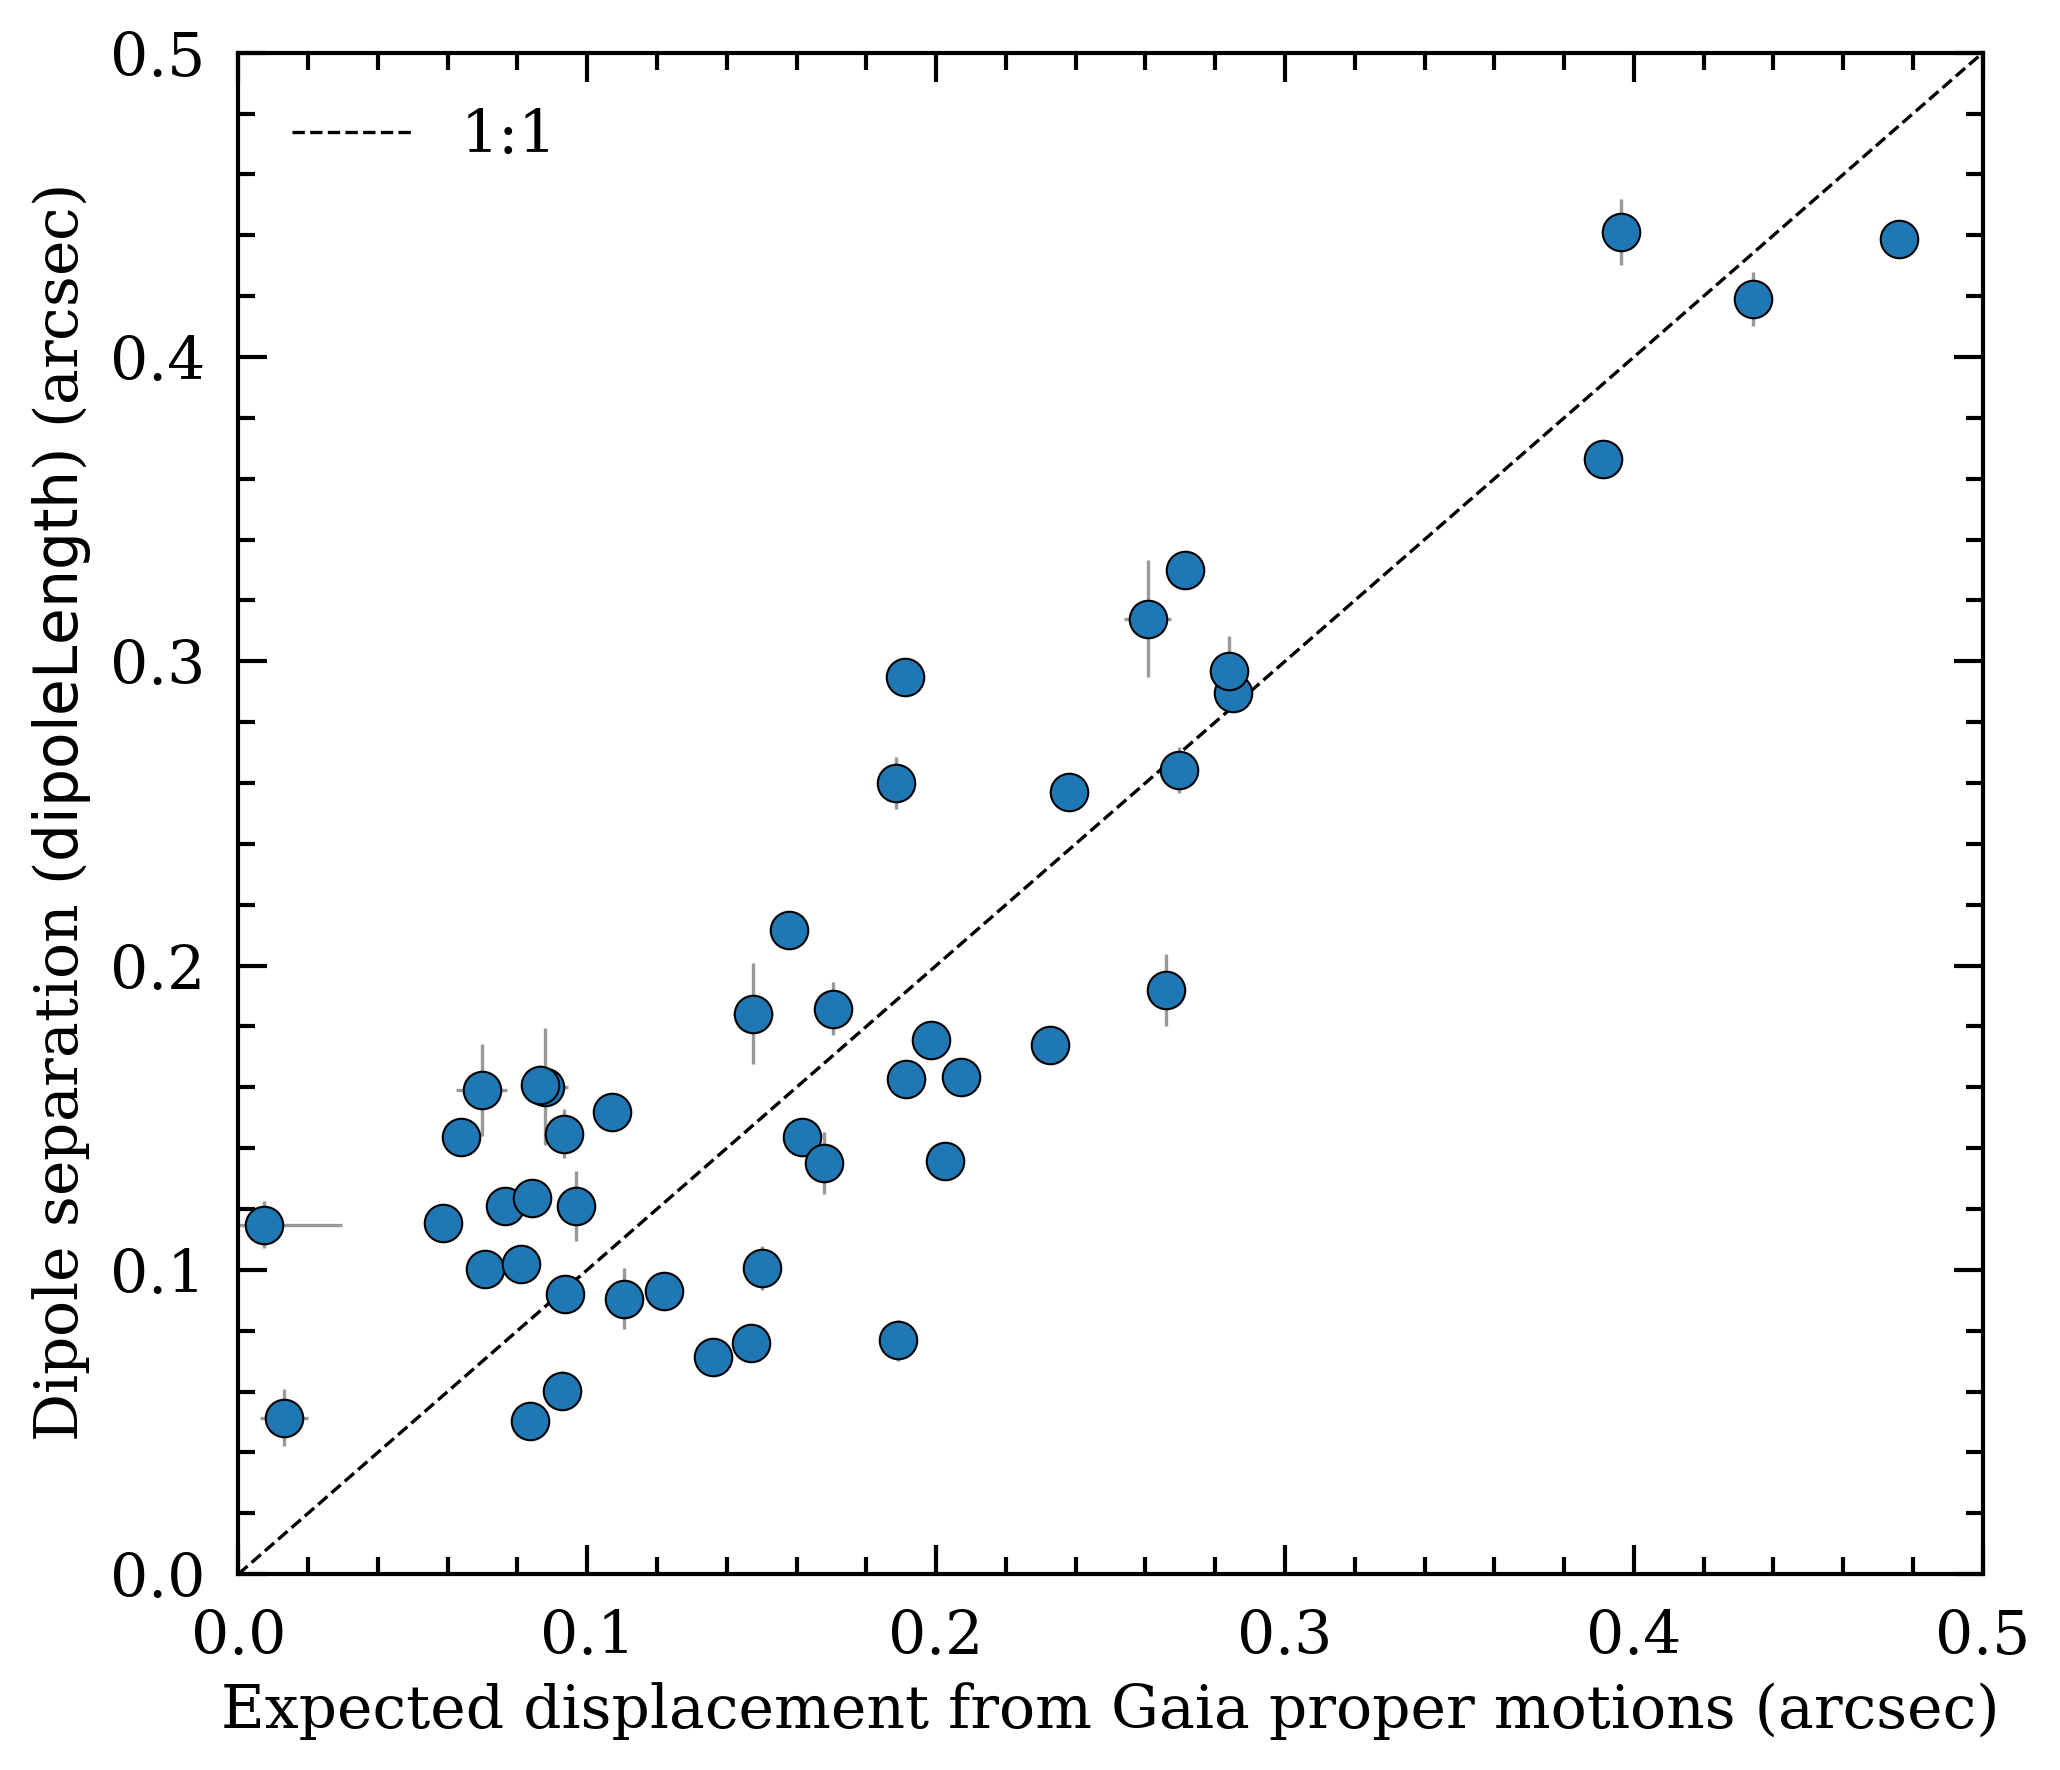
\includegraphics[width=0.65\linewidth]{figures/gaia_pms.png}
    \caption{The comparison of dipole separation measured by the pipeline dipole fit and the displacement expected from Gaia DR3 proper motion over the template-to-science interval of $\approx$10.62 years, for 46 DiaSources classified as dipoles and matched to Gaia stars with measured proper motions from one CCD difference image. The error bars show the errors on the proper motions and dipole separations obtained via error propagation from the errors on their individual components.
    }
    \label{fig:gaia_pms}
\end{figure}

\subsection{Long-term Variability}

Given the longer temporal baseline, slow-varying sources such as AGN are more likely to appear as significant difference image sources with DECam templates.
This corresponds to real astrophysical variation.

\subsection{Other Artifacts and Mismatches}




\subsection{Real-Bogus Performance}
\newpage
\appendix

\section{Acknowledgements}

This material is based upon work supported in part by the National Science Foundation through Cooperative Agreements AST-1258333 and AST-2241526 and Cooperative Support Agreements AST-1202910 and AST-2211468 managed by the Association of Universities for Research in Astronomy (AURA), and the Department of Energy under Contract No.\ DE-AC02-76SF00515 with the SLAC National Accelerator Laboratory managed by Stanford University.
Additional Rubin Observatory funding comes from private donations, grants to universities, and in-kind support from LSST-DA Institutional Members.

% Include all the relevant bib files.
% https://lsst-texmf.lsst.io/lsstdoc.html#bibliographies
\section{References} \label{sec:bib}
\renewcommand{\refname}{} % Suppress default Bibliography section
\bibliography{local,lsst,lsst-dm,refs_ads,refs,books}

% Make sure lsst-texmf/bin/generateAcronyms.py is in your path
\section{Acronyms} \label{sec:acronyms}
\input{acronyms.tex}
% If you want glossary uncomment below -- comment out the two lines above
%\printglossaries





\end{document}
